\documentclass[11pt,a4paper,twoside]{article}
\usepackage[utf8]{inputenc}
\usepackage{polski}

\usepackage{graphicx}
\usepackage{subcaption} % obrazki obok siebie
%\usepackage[caption=false]{subfig} % obrazki nad sobą
\usepackage{wrapfig} 
\usepackage{float}
\usepackage{geometry}
\usepackage{listings}
%\geometry{lmargin=3cm,rmargin=2cm, tmargin=2.5cm, bmargin=2.5cm} %marginesy w pracy inż/mgr
\geometry{lmargin=2.5cm,rmargin=2.5cm, tmargin=2.5cm, bmargin=2.5cm} %marginesy ogólne
\usepackage{multirow} % scalanie wierszy tabeli

\usepackage{fancyhdr}
\pagestyle{fancy}
\fancyhead{} % wszystkie nagłówki puste
%\fancyhead[RE,LO]{ Absolwenci Wydziału Prawa  2012}
\fancyfoot{} % wszystkie stopki puste
\fancyfoot[LE,RO]{\thepage}
\renewcommand{\headrulewidth}{0pt}
%\renewcommand{\footrulewidth}{0.4pt}

\usepackage[hidelinks]{hyperref}% nazwy odsyłaczy

%unikanie myślników dzielących słowa między liniami
\tolerance=1
\emergencystretch=\maxdimen
\hyphenpenalty=10000
\hbadness=10000

\usepackage{algorithm}
\usepackage{algorithmicx}
\usepackage{algpseudocode}
\makeatletter
\renewcommand{\ALG@name}{Algorytm}
\renewcommand{\figurename}{Wykres}

\usepackage{enumitem}
\setitemize{itemsep=1pt,topsep=1pt,parsep=1pt,partopsep=1pt} %odstępy wyliczanych elementów (-)

% \usepackage{indentfirst} % wcięcie w pierwszym akapicie (pod)rozdziału
\setlength\parindent{0pt}


%%%%%%%%%%%%%%%%%%%%%%%%%%%%%%%%%%%%%%%%%

%%% zawijanie tekstu w tabelach zgodnie z życzeniem
\usepackage{stackengine}
\usepackage{array}
\newcolumntype{L}[1]{>{\raggedright\arraybackslash}p{#1}}
\setstackEOL{\#}
\setstackgap{L}{12pt}
%%%

\usepackage{amsfonts} % zbiory liczba (np. naturalnych)
\usepackage{amsmath} %duże klamry
\usepackage{bbm} %skok jednostkowy
\usepackage[titletoc,title]{appendix} % dodatki - zmiana wyświetlania nagłówka
\pagenumbering{gobble}
\usepackage{afterpage} % pusta strona
\usepackage{tabularx}

\usepackage{makecell}
\usepackage{multirow}
\usepackage{array}
\newcolumntype{L}{>{\centering\arraybackslash}m{0.11\textwidth}}
\def\rot{\rotatebox}

\newcommand{\ten}[1]{$\cdot 10^{#1}$}
\newcolumntype{C}[1]{>{\centering\let\newline\\\arraybackslash\hspace{0pt}}m{#1}}
\usepackage{enumitem}
\renewcommand{\figurename}{Rys.}


\begin{document}
\pagenumbering{arabic}
\begin{center}
% \vspace*{3\baselineskip}
\LARGE{PRZETWARZANIE CYFROWE OBRAZÓW}\\
\LARGE{(POBR)}
\\
\vspace*{0.5\baselineskip}
{\LARGE{Projekt - rozpoznawanie loga mBanku}}
\\
\vspace*{0.5\baselineskip}
{\large{
Napieralski Adam
}}\\
\vspace*{0.5\baselineskip}
\large{\today}
\end{center}

\section{Temat projektu}
Dla indywidualnie wybranej klasy obrazów należało dobrać, zaimplementować i przetestować odpowiednie procedury wstępnego przetworzenia, segmentacji, wyznaczania cech oraz identyfikacji obrazów cyfrowych. Powstały w wyniku projektu program powinien poprawnie rozpoznawać wybrane obiekty dla reprezentatywnego zestawu obrazów wejściowych.

Wybrana klasa obrazów to zdjęcia zawierające logo mBanku (Rys. \ref{fig:logo_main}).

\begin{figure}[h]
    \centering
    
\includegraphics[height=2.5cm]{figures/mBank_logo_main.png}
    \caption{Logo mBanku}
    \label{fig:logo_main}
\end{figure}

\section{Wykorzystane narzędzia}
Projekt od strony technicznej został wykonany w języku \emph{C++}, posiłkując się ograniczonym zbiorem funkcji i obiektów z biblioteki \emph{OpenCV} (bez funkcji przetwarzania obrazu, wyłącznie podstawowe wczytywanie, zapis, wyświetlanie i struktury danych). Do budowy i kompilacji projektu wykorzystano narzędzie \emph{CMake}.
Instrukcja budowy i uruchomienia projektu znajduje się w pliku \emph{README.md} w plikach źródłowych.

\section{Charakterystyka wybranego logo}
Wybrane logo mBanku ma kształt prostokątny, złożone jest z:
\begin{itemize}
    \item pionowych pasów koloru: czerwonego, żółtego, zielonego, czarnego, niebieskiego;
    \item umieszczonego na nich białego napisu \emph{mBank}.
\end{itemize}

Jako najbardziej charakterystyczne cechy obrazu wybrane zostały trzy kolorowe pasy o największej powierzchni - czerwony, żółty i zielony. Ich bliskie siebie położenie oraz względnie niepowtarzalny kształt związany z nachodzeniem na nie białego napisu będą przydatne na etapie dalszego przetwarzania i ich wykrywania.

% \begin{figure}[H]
% \centering
% \begin{minipage}{.4\textwidth}
%   \centering
%   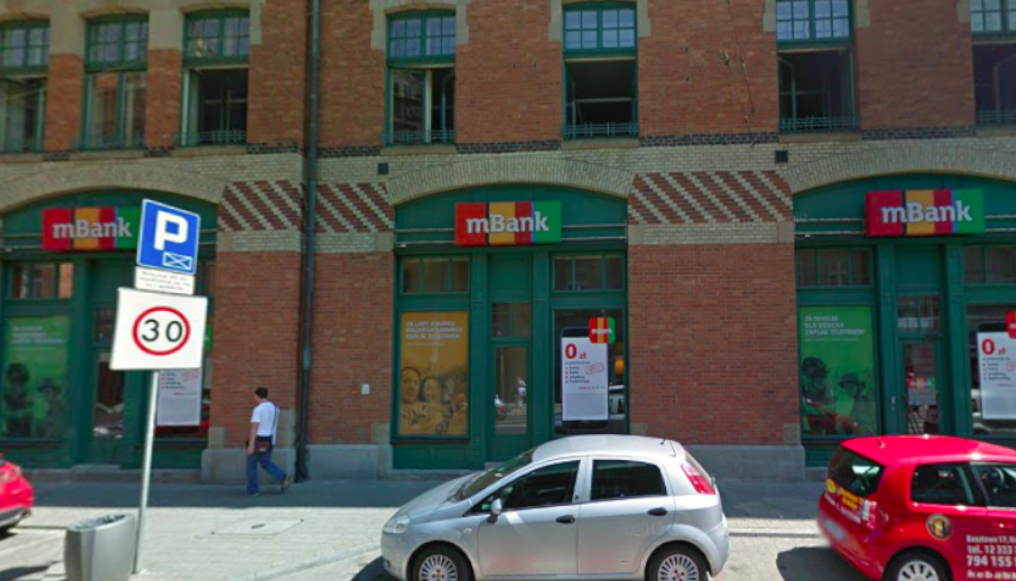
\includegraphics[width=\linewidth]{figures/img1.png}
%   \captionof{figure}{Wykres funkcji Rastrigina}
%   \label{fig:rastrigin}
% \end{minipage}%
% \begin{minipage}{.4\textwidth}
%   \centering
%   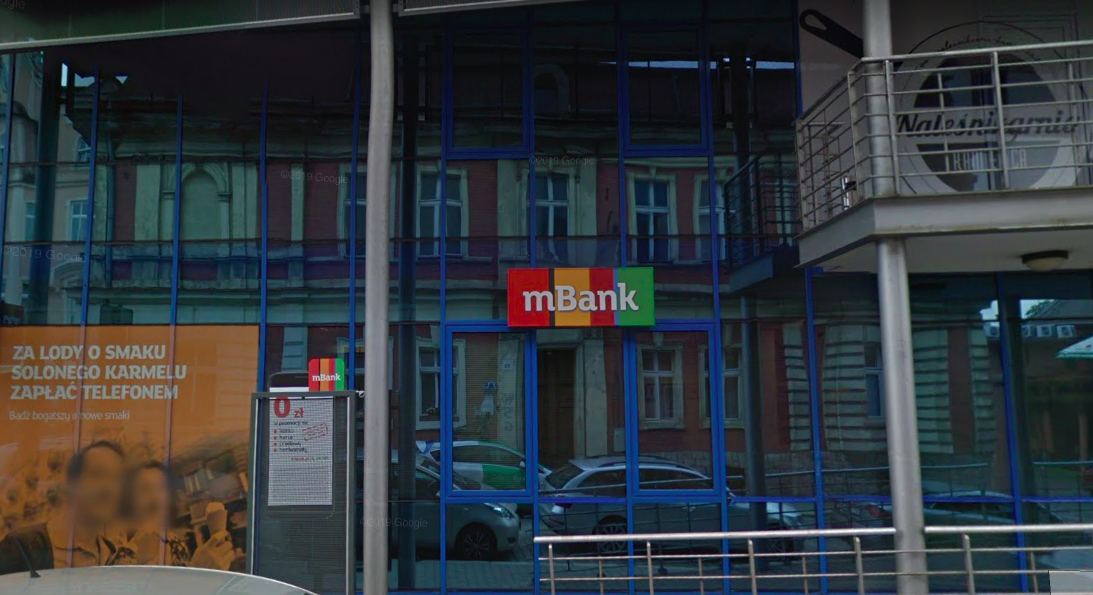
\includegraphics[width=\linewidth]{figures/img2.png}
%   \captionof{figure}{Wykres funkcji Schwefela}
%   \label{fig:schwefel}
% \end{minipage}
% \end{figure}

\begin{figure}[h]
\begin{subfigure}{.5\textwidth}
  \centering
  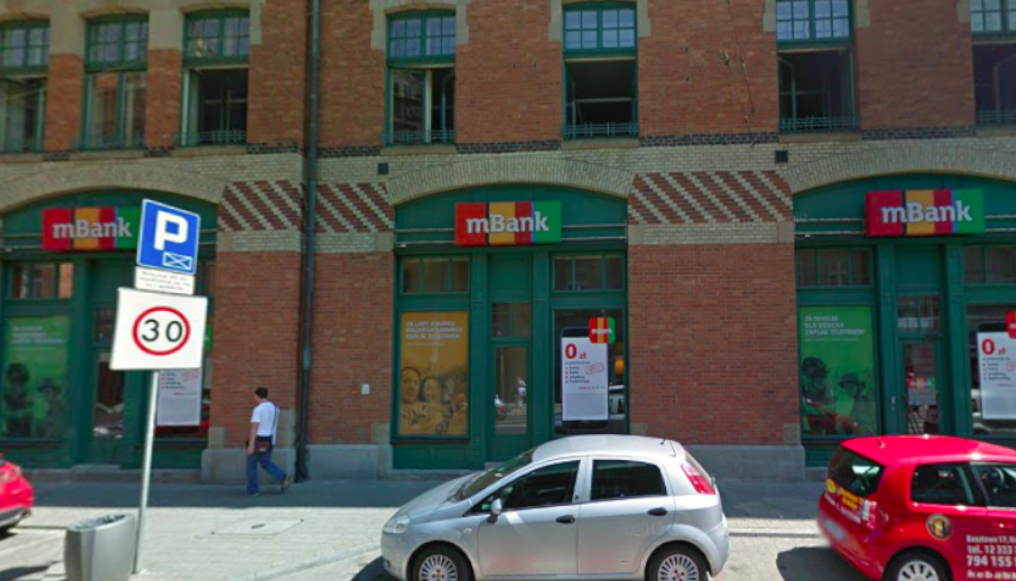
\includegraphics[width=.8\linewidth]{figures/img1.png}
  \caption{Obraz a}
  \label{fig:sfig1}
\end{subfigure}%
\begin{subfigure}{.5\textwidth}
  \centering
  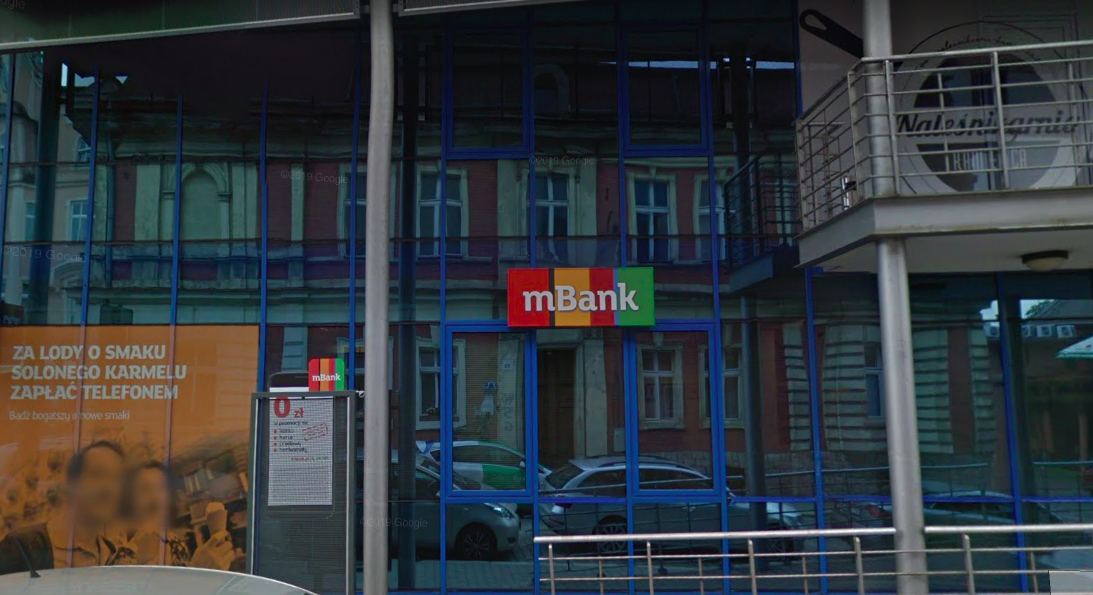
\includegraphics[width=.8\linewidth]{figures/img2.png}
  \caption{Obraz b}
  \label{fig:sfig2}
\end{subfigure}
\begin{subfigure}{.5\textwidth}
  \centering
  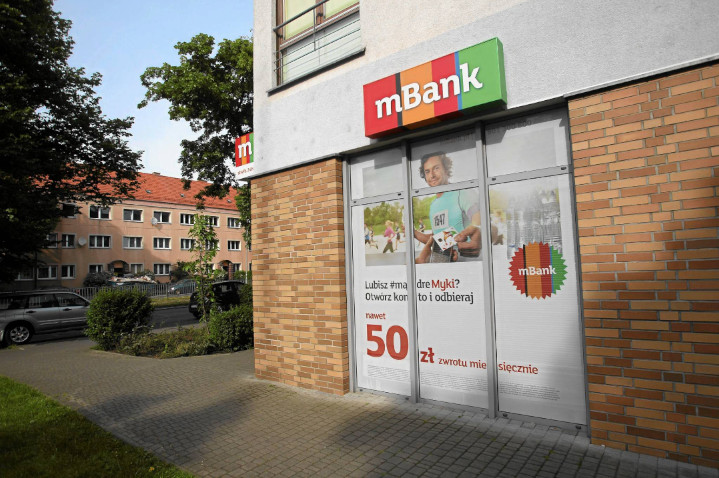
\includegraphics[width=.8\linewidth]{figures/img3.png}
  \caption{Obraz c}
  \label{fig:sfig2}
\end{subfigure}
\begin{subfigure}{.5\textwidth}
  \centering
  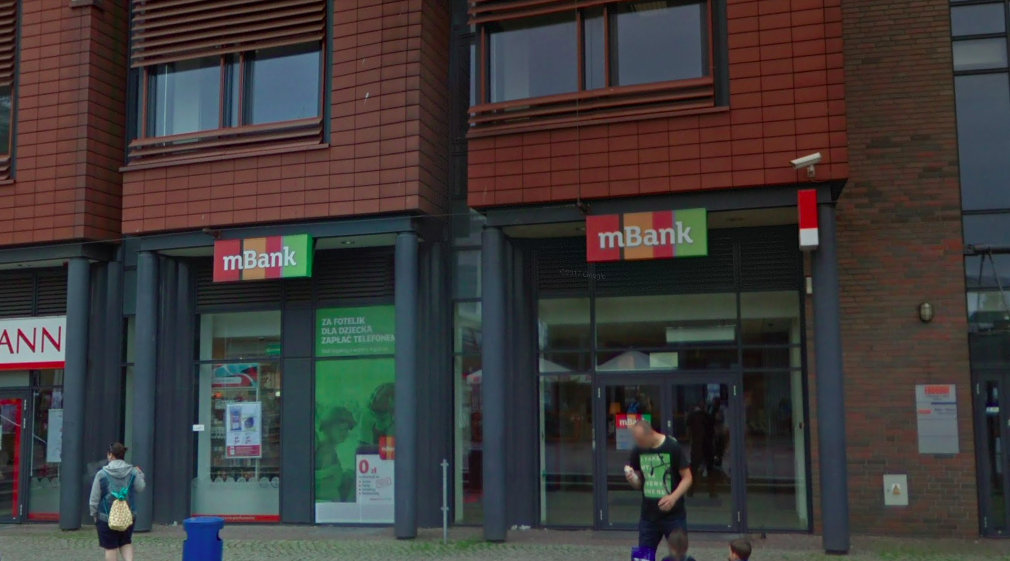
\includegraphics[width=.8\linewidth]{figures/img4.png}
  \caption{Obraz d}
  \label{fig:source-photos}
\end{subfigure}
\caption{Wybrane obrazy wejściowe}
\end{figure}

\section{Akwizycja obrazów wejściowych}
Jako zdjęcia wejściowe do tworzonego algorytmu przetwarzania i wykrywania logo wykorzystano obrazy:
\begin{itemize}
    \item naturalne - nie wygenerowane syntetycznie,
    \item z niejednorodnym tłem.
\end{itemize}
Jako obrazów użyto zdjęć pochodzących przede wszystkim z \emph{Google Street View}. Wybrano 4 obrazy (Rys. \ref{fig:source-photos}) - na dwóch z nich znajduje się po jednym logo, na pozostałych znajdują się po 2 i po 3.


\section{Zarys algorytmu przetwarzania}
W zaproponowany algorytmie wykrywania logo mBanku można wyróżnić 4 podstawowe kroki przetwarzania obrazu:
\begin{enumerate}[topsep=1pt,itemsep=0ex,partopsep=1ex,parsep=1ex]
    \item Konwersja przestrzeni barw.
    \item Segmentacja.
    \item Wyznaczanie cech.
    \item Identyfikacja.
\end{enumerate}
Każdy z nich zostanie bliżej omówiony, przedstawione zostaną wybrane szczegóły implementacyjne oraz wnioski wyniesione na podstawie wykonanych prac.
% \begin{algorithm}[ht]
% \label{image-processing}
% 	\begin{algorithmic}
% 	\State{1. Konwersja przestrzeni barw.}
% 	\State{2. Progowanie.}
% 	\State{3. Segmentacja.}
% 	\State{4. Wyznaczanie cech.}
% 	\State{5. Identyfikacja.}
% 	\end{algorithmic}
% \end{algorithm}

\section{Przetwarzanie wstępne}
Do etapu przetwarzania wstępnego zaimplementowano algorytmy rozmycia i wykrywania krawędzi obrazu - przy pomocy filtru dolno- i górnoprzepustowego. Na etapie eksperymentalnym zaobserwowano jednak, że obrazy wejściowe w swojej domyślnej formie lepiej sprawdzają się w detekcji, przez co użycie filtrów stało się niekonieczne, przez co we właściwym procesie nie zostały wykorzystane. Efekty ich działań w celach poglądowych zaprezentowano jednak na Rys. \ref{fig:filtry}.

\begin{figure}[H]
\begin{subfigure}{.5\textwidth}
  \centering
  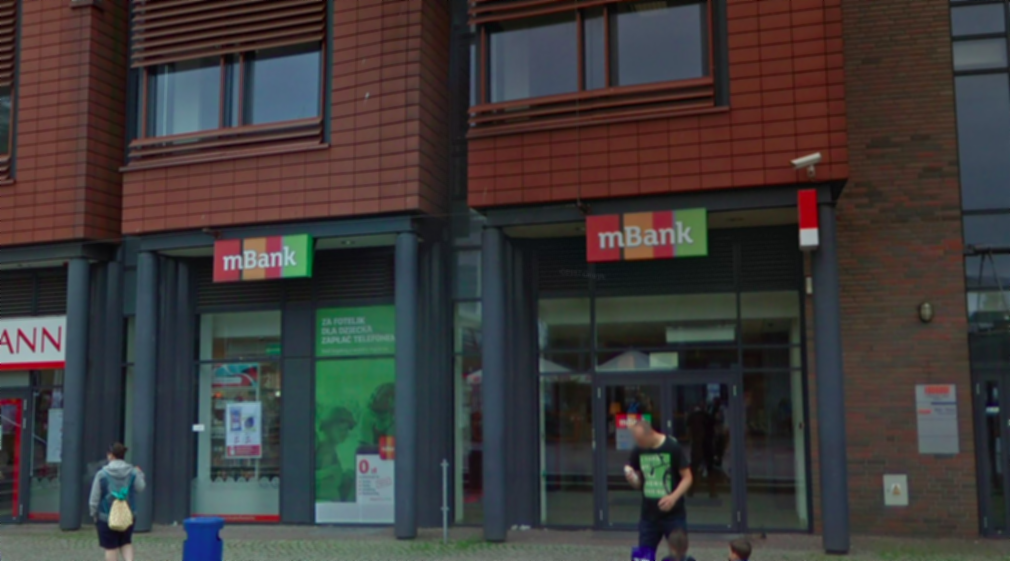
\includegraphics[width=.8\linewidth]{figures/img_blurred.png}
  \caption{Filtr dolnoprzepustowy - rozmycie}
  \label{fig:sfig1}
\end{subfigure}%
\begin{subfigure}{.5\textwidth}
  \centering
  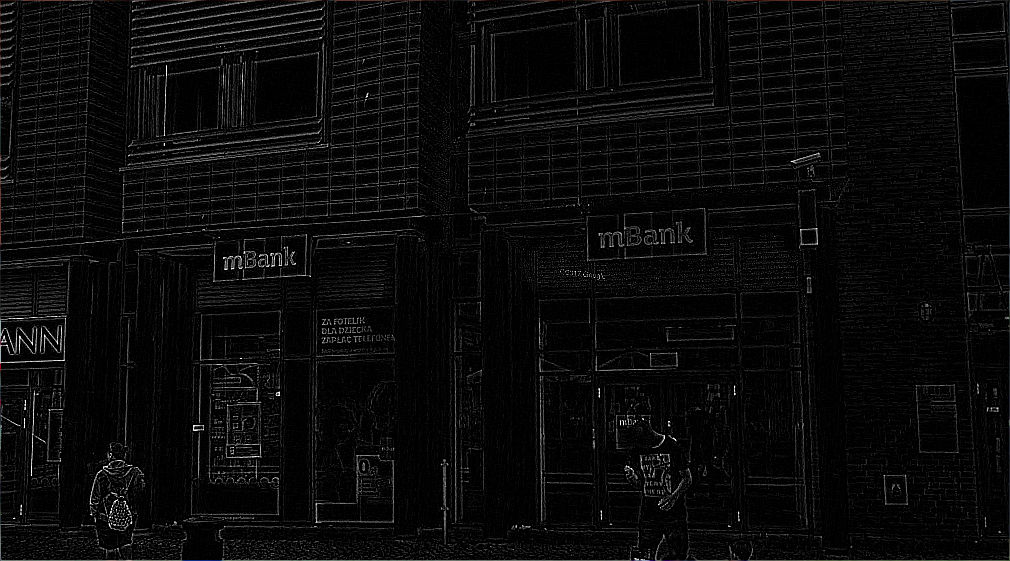
\includegraphics[width=.8\linewidth]{figures/img_sharpened.png}
  \caption{Filtr górnoprzepustowy - zaznaczenie krawędzi}
  \label{fig:sfig2}
\end{subfigure}
\caption{Efekty działania zaimplementowanych filtrów na obrazie d}
\label{fig:filtry}
\end{figure}

\section{Konwersja przestrzeni barw}
Wejściowy obraz zapisany jest w formacie \emph{RGB} (a właściwie \emph{BGR} - z racji wykorzystania wczytywania z użyciem biblioteki \emph{OpenCV}). W celu łatwiejszej selekcji interesujących pikseli na etapie progowania zdecydowano się na konwersję przestrzeni barw do przestrzeni \emph{HSV}.

Zaimplementowany algorytm konwersji bazuje na odpowiadającej mu metodzie z \emph{OpenCV}.

\begin{equation}
    \label{eqn:value}
    V = \max{(R, G, B)}
\end{equation}

Kolejnym krokiem algorytmu, jest obliczenie nasycenia koloru $S$, korzystając ze wzoru~\ref{eqn:saturation}.

\begin{equation}
    \label{eqn:saturation}
    S = \left\{ 
        \begin{array}{ll}
            0, & V = 0 \\
            \min{(R, G, B)}, & V \ne 0
        \end{array} 
        \right.
\end{equation}

Ostatnim krokiem algorytmu jest obliczenie barwy $H$~zgodnie z~wzorem~\ref{eqn:hue}.

\begin{equation}
    \label{eqn:hue}
    H = \left\{ 
        \begin{array}{ll}
            \frac{(G - B) * 60^{\degree}}{V - \min{(R, G, B)}} + 60^{\degree}, & V = R \\
            \frac{(B - R) * 60^{\degree}}{V - \min{(R, G, B)}} + 120\si{\degree}, & V = G \\
            \frac{(R - G) * 60^{\degree}}{V - \min{(R, G, B)}} + 240^{\degree}, & V = B
        \end{array} 
        \right.
\end{equation}
Tak uzyskane wartości parametrów S i V zawierają się w przedziale $[0, 255]$, natomiast parametr H, z racji przechowywania go jako 8-bitowej liczby, skalowany jest z typowego zakresu $[0, 359]$ do $[0, 179]$.
Operacja konwersji przestrzeni barw jest operacją punktową, przez co może być realizowana na każdym pikselu osobno, niezależnie od innych, sąsiednich.
W programie za ten etap przetwarzania odpowiadają klasy: \emph{BGR2HSVConverter} i \emph{BGR2HSVPixelConverter}.


\section{Segmentacja}
Na etapie segmentacji skorzystano z dwóch jej różnych typów, mających w końcowym efekcie oznaczyć obszary obrazu jednorodne pod określonymi cechami.

\subsection{Segmentacja punktowa - progowanie}
W celu wyselekcjonowania pikseli należących do jednego z trzech wybranych obszarów zainteresowania należących do loga zastosowano metodę progowania na wcześniej przekonwertowanym do przestrzeni HSV obrazie. 
Drogą eksperymentalną wybrano progi dla każdej z trzech rozważanych barw - przedziały wartości parametrów H, S, V - które przedstawiono w Tabeli \ref{tab:progi}.

\begin{table}[h]
\centering
\begin{tabular}{c|c|c|c|c|c|c}
    Kolor & $H_{\mathrm{min}}$ & $H_{\mathrm{max}}$ & $S_{\mathrm{min}}$ & $S_{\mathrm{max}}$ & $V_{\mathrm{min}}$ & $V_{\mathrm{max}}$ \\ \hline 
    czerwony 1 & $ 150 $ & $179$ & $110$ & $255$ & $90$ & $255$ \\ \hline
    czerwony 2 & $0$ & $3$ & $110$ & $255$ & $90$ & $255$ \\ \hline
    żółty & $9$ & $22$ & $60$ & $255$ & $80$ & $255$ \\ \hline
    zielony & $25$ & $87$ & $70$ & $255$ & $80$ & $255$\\
\end{tabular}
\caption{Tabela wybranych progów}
\label{tab:progi}
\end{table}

Przetwarzanie progowania zawarte zostało w plikach \emph{Binarization}, a główną funkcją je realizującą jest \emph{inRange} - analogiczna do funkcji o tej samej nazwie z biblioteki \emph{OpenCV}. Z funkcji zwracany jest zbinaryzowany obraz, gdzie piksele należące do wybranego przedziału oznaczone są na biało (wektorem wartości [255, 255, 255]), a pozostałe na czarno ([0, 0, 0]).

Ponieważ dla koloru czerwonego wartości progów dla parametru H przechodziły przez skrajne możliwe wartości (0 i 179), przeprowadzono osobne progowanie dla obu wariantów i tak uzyskane obrazy scalono w jeden wykorzystując operację logicznego \emph{OR} na pikselach.

Wyniki działania progowania przedstawiono na Rys. \ref{fig:progowanie_kolory}. 

\begin{figure}[h]
\centering
\begin{subfigure}{.3\textwidth}
  \centering
  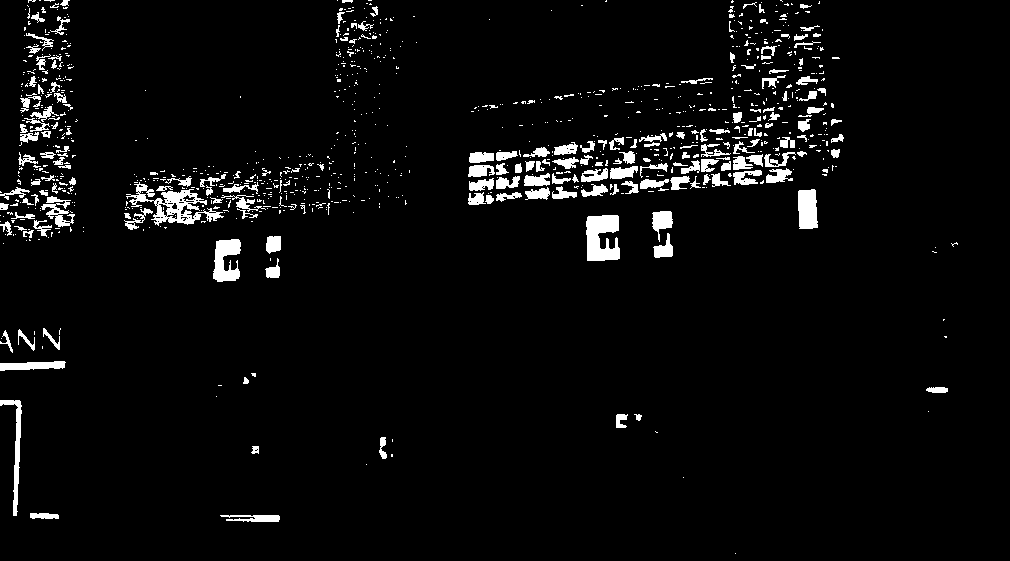
\includegraphics[width=.8\linewidth]{figures/img4_thresh_red.png}
  \caption{Czerwony}
  \label{fig:sfig1}
\end{subfigure}
\begin{subfigure}{.3\textwidth}
  \centering
  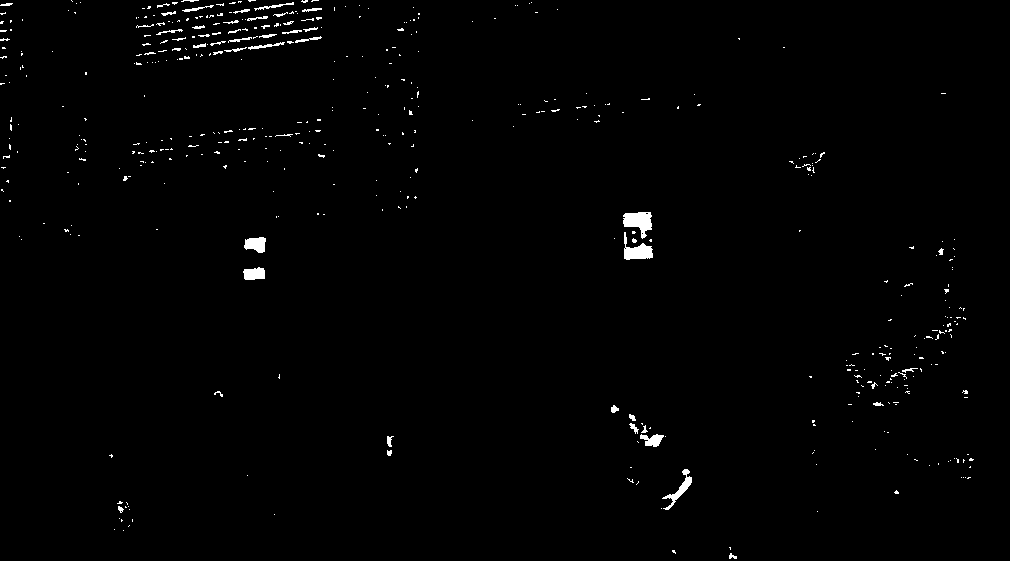
\includegraphics[width=.8\linewidth]{figures/img4_thresh_yellow.png}
  \caption{Żółty}
  \label{fig:sfig2}
\end{subfigure}
\begin{subfigure}{.3\textwidth}
  \centering
  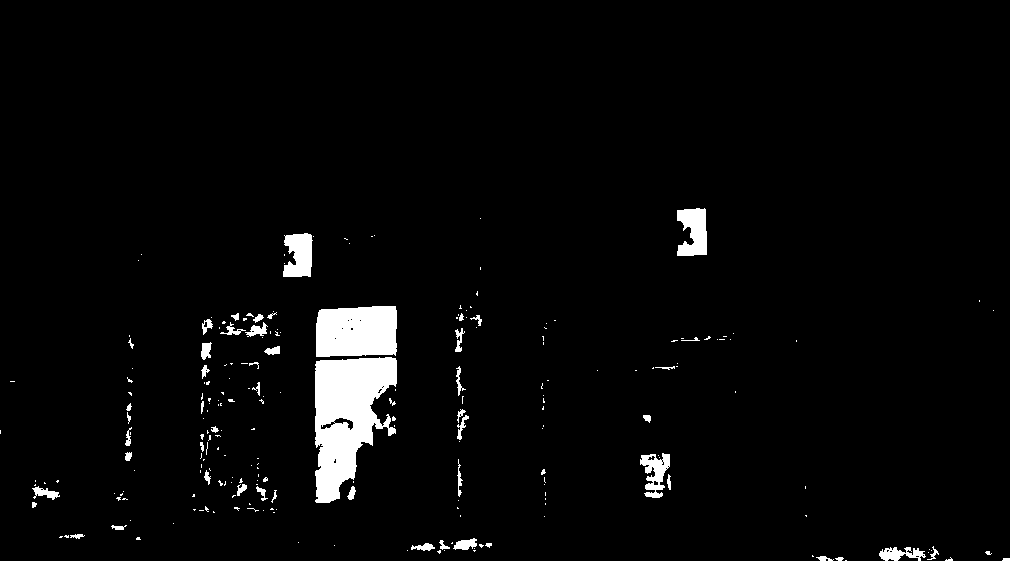
\includegraphics[width=.8\linewidth]{figures/img4_thresh_green.png}
  \caption{Zielony}
  \label{fig:sfig2}
\end{subfigure}
\caption{Binarne obrazy uzyskane po zastosowaniu progowania na obrazie \empty{d} dla poszczególnych kolorów}
\label{fig:progowanie_kolory}
\end{figure}

\subsection{Segmentacja obszarowa - rozrost obszarów}

Na tym etapie przetwarzania z jednostkowe piksele oznaczone na etapie progowania zostały pogrupowane w większe segmenty. Dokonano tego stosując implementując algorytm podążający za ogólną zasadę algorytmów typu \emph{flood fill}.

Rozpoczynając grupowanie od jednego znalezionego zaznaczonego piksela, analizowano rekursywnie sąsiadów kolejnych pikseli. Wybranym wariantem sąsiedztwa pikseli został wariant 4-pikselowy (przedstawiony na Rys. \ref{fig:pixel_4_nb}).

\begin{figure}
    \centering
    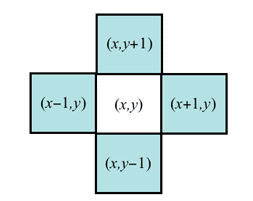
\includegraphics[width=5cm]{figures/4_pixel_neighbourhood.png}
    \caption{Wybrany wariant określający sąsiedztwo piksela}
    \label{fig:pixel_4_nb}
\end{figure}


\section{Identyfikacja}
W celu rozpoznania całego logo oparto się na identyfikacji cech wyznaczonych segmentów składowych: jednego czerwonego, żółtego i zielonego. By to osiągnąć skorzystano z parametrów, które w trakcie analizy dawały najbardziej charakterystyczne dla danych segmentów wyniki. Wybrano: niezmienniki momentowe \emph{NM1} i \emph{NM7} oraz współczynnik \emph{W3}  - Malinowskiej, którego wzór wygląda następująco:
\begin{equation}
    W3=\frac{L}{2\sqrt{\pi}S}-1
\end{equation}
\begin{center}
    gdzie $L$ - obwód segmentu, $S$ - jego pole.
\end{center}

Dla każdego z nich metodą eksperymentalną wyznaczono przedziały wartości - przedstawione w Tab.. Segment, którego wszystkie wartości współczynników będą należały do tych przedziałów zostanie zaklasyfikowany jako prawdopodobny segment składowy identyfikowanego logo (Rys. \ref{fig:segmenty_kolorow_poszczegolnych}).

\begin{table}[H]
    \centering
    \begin{tabular}{|c|c|c|c|}
    \hline
         Segment & NM1 & NM7 & W3 \\
         \hline
         czerwony & $[0,21, 0,28]$ & $[0,011, 0,014]$ &  $[0,66, 1,85]$\\
         \hline
         żółty & $[0,18, 0,38]$ & $[0,005, 0,022]$ &  $[0,75, 1,75]$\\
         \hline
         zielony & $[0,18, 0,34]$ & $[0,007, 0,12]$ &  $[0,45, 2,51]$\\
         \hline
    \end{tabular}
    \caption{Przedziały wartości wybranych współczynników charakterystycznych dla segmentów składowych logo}
    \label{tab:przedzialy_wspolczynnikow}
\end{table}

\begin{figure}[H]
\centering
\begin{subfigure}{.3\textwidth}
  \centering
  
\includegraphics[width=.8\linewidth]{figures/img4_thresh_colored_red.png}
  \caption{Czerwony}
  \label{fig:sfig1}
\end{subfigure}
\begin{subfigure}{.3\textwidth}
  \centering
  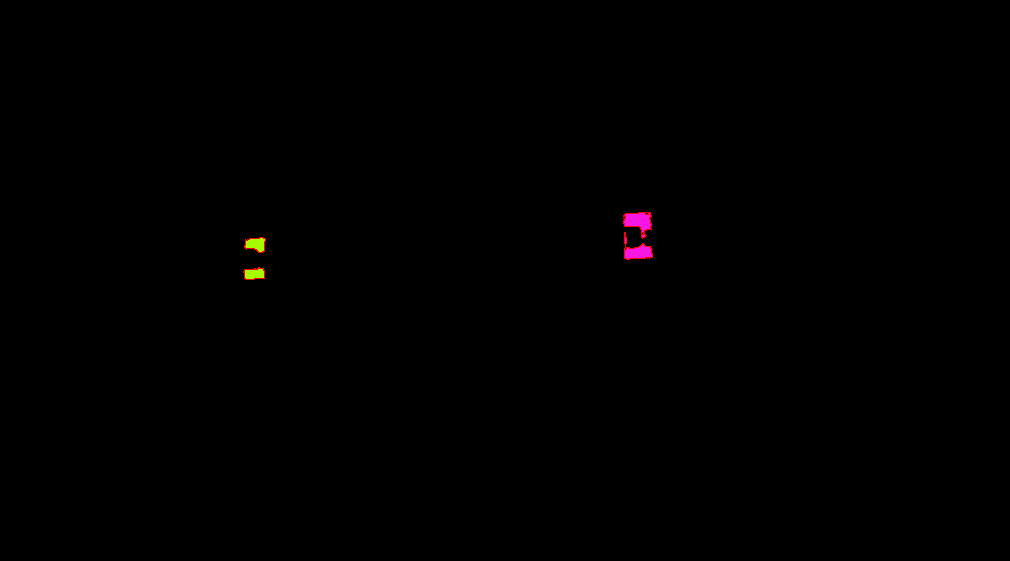
\includegraphics[width=.8\linewidth]{figures/img4_thresh_colored_yellow.png}
  \caption{Żółty}
  \label{fig:sfig2}
\end{subfigure}
\begin{subfigure}{.3\textwidth}
  \centering
  
\includegraphics[width=.8\linewidth]{figures/img4_thresh_colored_green.png}
  \caption{Zielony}
  \label{fig:sfig2}
\end{subfigure}
\caption{Zaznaczone zidentyfikowane segmenty na obrazie \empty{d} dla poszczególnych kolorów}
\label{fig:segmenty_kolorow_poszczegolnych}
\end{figure}

Ostatecznym krokiem to identyfikacji samego logo jest przeszukanie kolekcji wszystkich wykrytych 3 typów segmentów i określenie położenia logotypu na podstawie względnego położenia 3 typów segmentów. Wykonywane jest to przy pomocy metody \textit{LogoRecognizer::findLogos}, a kryterium poprawnego zaklasyfikowania 3 segmentów jako składowe jednego logo jest wzajemna bliskość ich geometrycznych środków przy współczynniku $1,5$, określającym mnożnik długości przekątnej prostokąta opisanego na segmencie, który następnie traktowany jest jako promień koła wyznaczającego obszar sąsiedztwa danego segmentu. Tak pogrupowane segmenty są następnie łączone w jeden, który reprezentuje faktyczne zidentyfikowane logo (Rys. \ref{fig:segmenty_wszystkich_kolorow}).

\begin{figure}[H]
    \centering
    
\includegraphics[width=10cm]{figures/img4_thresh_all_colored.png}
    \caption{Oznaczone segmenty połączone w jeden określający faktyczne zidentyfikowane logo}
    \label{fig:segmenty_wszystkich_kolorow}
\end{figure}


\section{Uzyskane wyniki}
W ramach projektu dokonano analizy 4 zdjęć, z czego na dwóch z nich logo pojawiało się wielokrotnie. Na wszystkich udało się rozpoznać wszystkie logotypy mBanku.

\begin{figure}[h]
\begin{subfigure}{.5\textwidth}
  \centering
  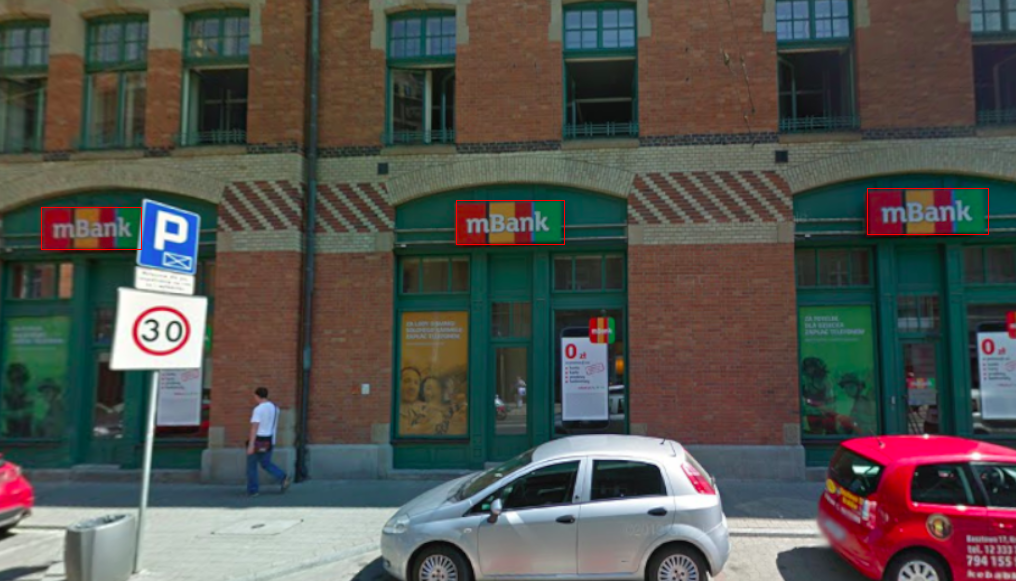
\includegraphics[width=.8\linewidth]{figures/img1_marked_out.png}
  \caption{Obraz a}
  \label{fig:sfig1}
\end{subfigure}%
\begin{subfigure}{.5\textwidth}
  \centering
  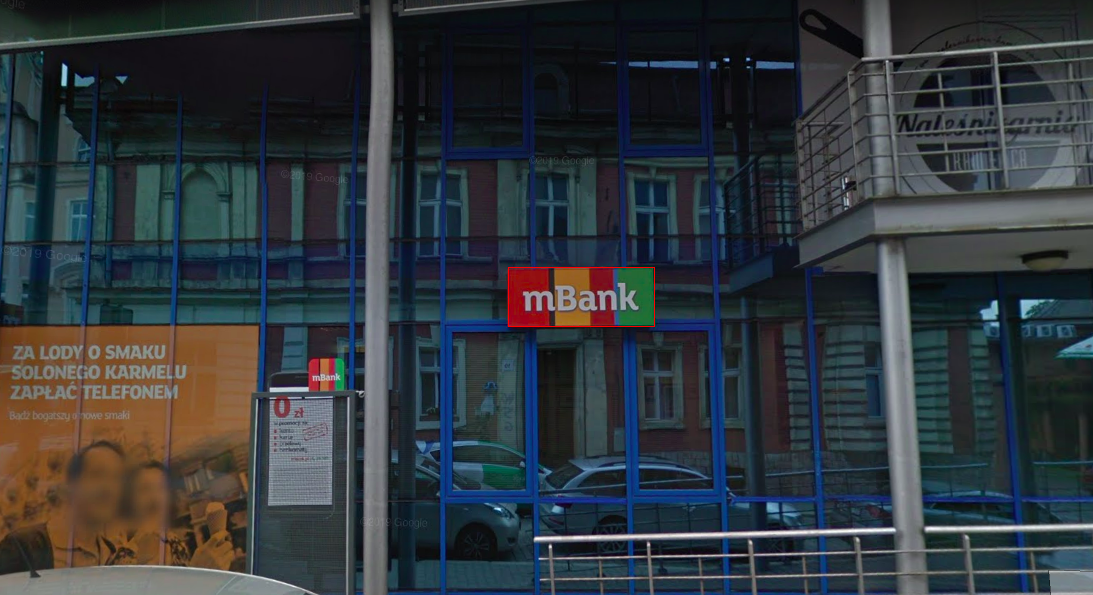
\includegraphics[width=.8\linewidth]{figures/img2_marked_out.png}
  \caption{Obraz b}
  \label{fig:sfig2}
\end{subfigure}
\begin{subfigure}{.5\textwidth}
  \centering
  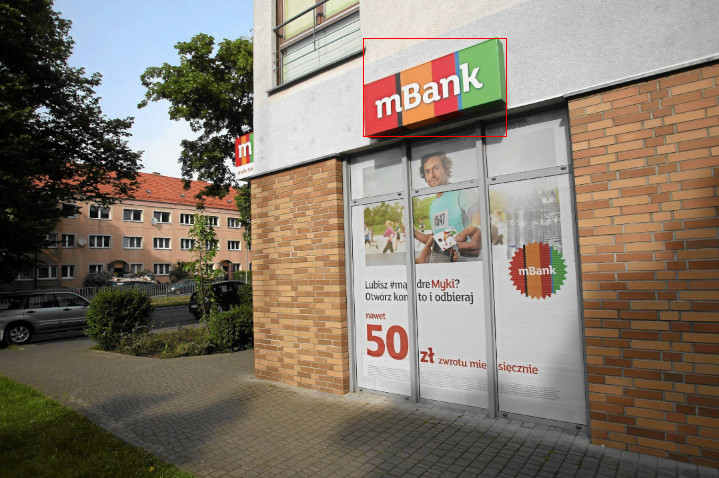
\includegraphics[width=.8\linewidth]{figures/img3_marked_out.png}
  \caption{Obraz c}
  \label{fig:sfig2}
\end{subfigure}
\begin{subfigure}{.5\textwidth}
  \centering
  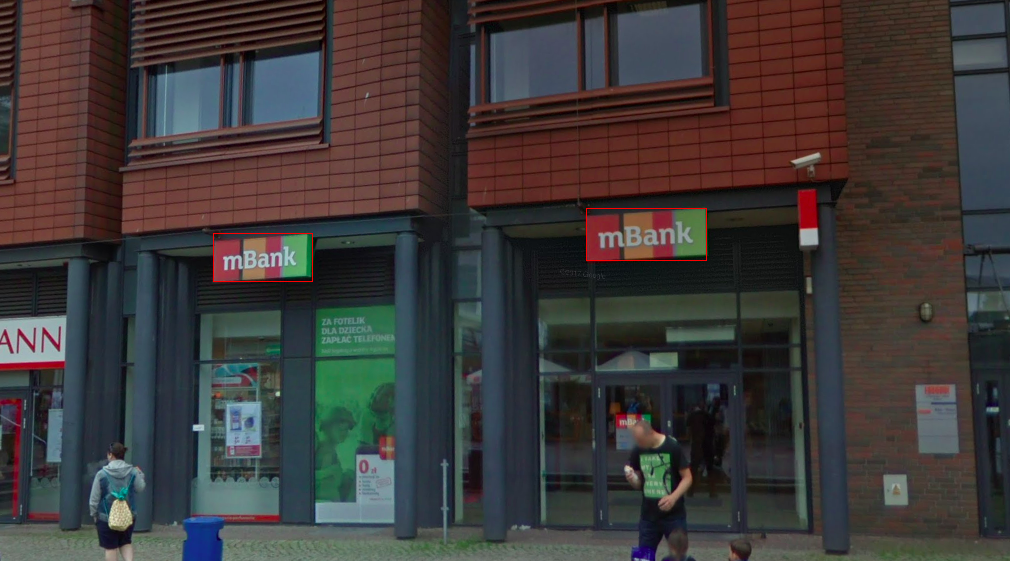
\includegraphics[width=.8\linewidth]{figures/img4_marked_out.png}
  \caption{Obraz d}
  \label{fig:source-photos}
\end{subfigure}
\caption{Analizowane obrazy z zaznaczonymi wykrytymi logotypami}
\end{figure}

\newpage





\begin{thebibliography}{9}
\bibitem{img-segm}
Image segmentation
\url{https://www.cs.auckland.ac.nz/courses/compsci773s1c/lectures/ImageProcessing-html/topic3.htm}
\bibitem{wyklady}
prof. Przemysław Rokita. Wykłady z przedmiotu przetwarzanie obrazów cyfrowych

\end{thebibliography}
\end{document}